\section{Methods}

\subsection{Naive Bayes}
% mention prior

The problem can be defined as a text classification problem with the verbs as labels and the subject and object as features. For each SVO document, the number of features is fixed as two. According to the Naive Bayes conditional independency assumption, given the subject s and the object o, the Naive Bayes formula to predict verb $v$ is provided as below.

\begin{equation}
	\hat{v} = \arg\max_v P(v|so) = \arg\max_v P(v)P(s|v)P(o|v)
\end{equation}

One thing we notice here is that the subject and the object are not symmetric. "Cat eat fish" and "Fish eat cat" should not be considered equal. Based on this intuition, we have two different subject and 

However, there exist duplicated features with different labels. For example, a "cat" can eat "fish", and can also like a "fish". As a classifier, Naive Bayes only gives the label with the highest conditional probability. It doesn't produce multi labels results for a given input document. In our experiments, when the system make a prediction that is one of the correct labels, there will be one "true positive" and all other possible correct answers will be marked as "false negative".

\subsection{Scalability}

Conventional Naive Bayes implementations stores a structure the size of \\
\\
$|Features| * |Label|$ \\
\\
in memory. In our case, this would be a \\
\\
$(|Subject\_Categories|+|Unique\_Subject|\\+|Object\_Categories|+|Object\_Subject|) * |Verbs|$ \\

sized structure. This is unfeasible for the amount of data we are working with. To deal with such a large volume of data we proposed a Naive Bayes algorithm in MapReduce implemented in Hadoop. This method of Naive Bayes is similar to Streaming Naive Bayes and does not require large global structures to be kept.\\
\\
At a high level, this requires going over the data 4 times. Once to count the number of occurrences of each verb. Once to count the number of occurrences of each Subject, Object and their categorical counts. Once to train. Once to test and evaluate the results. At the end of each phase, we store some small statistics into the context of our map and reduce jobs such as the number of unique subjects, objects, ontology for the next task.\\
\\
We only need to transform counts into conditional probabilities in the testing phase, since conditional probabilities are only needed for each test example. We can do a map emitting $<$Subject\/Object, [TestNum, test\_counts, train\_counts]$>$. This way we can parallelize to the full extent by putting all necessary information to calculate conditional probabilities in the reducer for a given Subject or Object.

This implementation scales well with the task because there are a lot of different possible subjects and objects. Since almost every map phase emits the subject or object as the key, the problem can easily be parallelized. The limit is not reached until the number of reducers equals the number of unique keys.

\subsection{Stemming}

The dataset from SVO tuples are parsed from sentences and not stemmed. Stemming can help to merge different tuples and reduce both feature set size and label set size. However, considering the database for ontology contains unstemmed words, we can't stem the subject and object words in the data file because that stemming will increase the ontology matching failure rate.

Despite of that, verbs can be stemmed to reduce the possible label set size. Stemmed verbs can cannonicalize verbs that actually mean the same thing but are in different tense, for example \emph{provides} vs. \emph{provided}. This can reduce number of labels, prediction error, and also the size of the intermediate data. We used a simple \emph{Porter Stemmer} for this task.
% left to Yilun

\subsection{Smoothing}

Considering the sparsity of language models, the \emph{Maximum-likelihood Estimator} version of Naive Bayes would likely result in a posterior probability of zero. A Dirichlet prior is often used. The Dirichlet prior pulls the features to a uniform distribution at a certain strength according to parameter $\alpha$. In many cases, as a simplification, plus one smoothing is used as a simplified Dirichlet prior with $\alpha=1$.

\subsection{Categorical Smoothing}

\begin{figure}[ht]
\vskip 0.2in
\begin{center}
\centerline{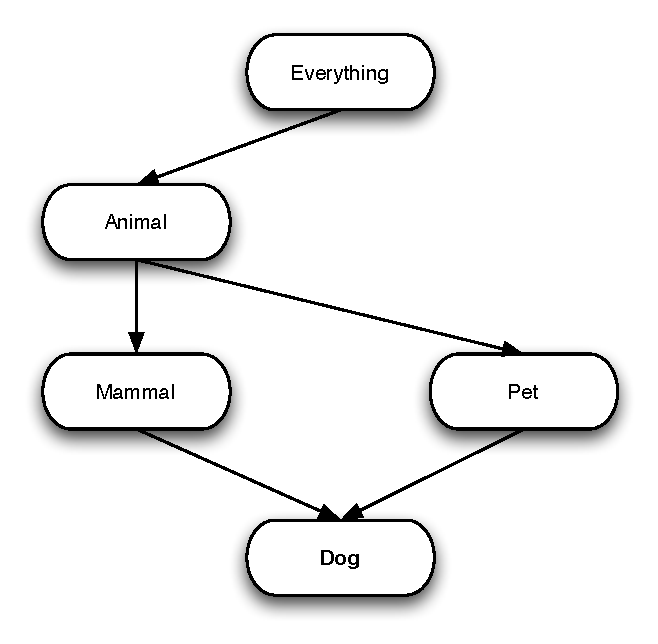
\includegraphics[width=\columnwidth]{dog}}
\caption{Categories for Dog}
\label{fig-dog-category-example}
\end{center}
\vskip -0.2in
\end{figure}

As mentioned before, NELL has a knowledge base with ontology information for many known entities. Usually more than one categories are provided for nouns. For example, a dog is a mammal, an animal, an everything and a pet. Some of the categories have containing relations. For the ``dog" example, we can describe the category relation as figure \ref{fig-dog-category-example}. As is shown in the figure, some categories like "mammal" are very close to the entity thus describe some attributes of the entity while others like "everything" are very faraway and thus not informative. In our observations, one degree parent categories are usually more helpful.

% \begin{figure}[ht]
% \vskip 0.2in
% \begin{center}
% \centerline{\includegraphics[width=\columnwidth]{icml_numpapers}}
% \caption{Historical locations and number of accepted papers for International
%   Machine Learning Conferences (ICML 1993 -- ICML 2008) and
%   International Workshops on Machine Learning (ML 1988 -- ML
%   1992). At the time this figure was produced, the number of
%   accepted papers for ICML 2008 was unknown and instead estimated.}
% \label{fig-dog-category-example}
% \end{center}
% \vskip -0.2in
% \end{figure}

In order to use the category information in the Naive Bayes model, we considered two approaches. One naive approach is to add category counts as independent features. In this way we increase the number of features for each document to above 4. However, this implementation heavily violates the strong dependent nature of these features. If a ``dog" is in the feature set, ``mammal" and ``pet" must also be in the feature set. But ``dog'', ``mammal'', and ``pet'' are highly correlated in reality. This means the model will have very high bias to begin with and probably will not work well.

Instead, we propose another approach, which is also our core contribution to this work. We introduce \emph{categorical smoothing}.\\

Recall with Laplace smoothing, we can say that we assume each word appears in each label approximately $\frac{1}{|w|}$ times with $\alpha = 1$.\\

\begin{equation}
	P(w|L) = \frac{Count(w|L)+\alpha}{Count(L)+\alpha |w|}
\end{equation}

With categorical smoothing, we know that the word is a member of a given category, thus its category can represent this word, so we assume that they appear $\frac{category(w)}{|categories|}$ of times. 

\begin{equation}
	P(w|L) = \frac{Count(w|L)+\alpha Count(category(w))}{Count(L)+\alpha \sum_i(category(i))}
\end{equation}

This method of smoothing takes independence of what the actual label is. It is a way to differentiate  where the different categories subjects and objects come from. Beliefs within the same category will not be effected by this type of smoothing because the weights applied are the same and hence only $Count(w|L)$ differentiates, but beliefs from different categories will be heavily influenced by this smoothing.

\subsection{Label Set}

As mentioned earlier, our label set is \emph{Verbs} that relate the subject and the object. There is non trivial number of verbs that can relate subjects and objects, hence the possible label space we expect to label is also quite large. We will do classification with controlled numbers of verbs/labels. Though we do expect that as the number of labels grow, the variance of the data will grow and that our classifiers will naturally become not as accurate.

\subsection{Evaluation and Metric}

We use NELL beliefs as labeled true data for training and testing. $10\%$ data is held out for test purpose and the other $90\%$ is training set. Cross validation could be a more useful technique but we don't intend to use it because it will require repetitive runs over the data and will be very computationally costly.

As a single-label prediction problem, we use precision as the metric to evaluate the classifier. According to the definition of precision,

\begin{equation}
	p = \frac{number_{truePositive}}{number_{truePositive} + number_{falsePositive}}
\end{equation}

Besides, different verbs for the same pair of subject and object are considered as different test cases. Since our system always predict one verb for a given subject-object pair, we always lose precision and recall on multi-label cases. Actually, considering it's a single-label prediction on a multi-label dataset, the precision is always equal to the recall.




